\documentclass[a4paper,12pt]{article}
\usepackage{graphicx} 			% Para insertar imagenes
\usepackage{indentfirst} 	% Para sangrar párrafos después de secciones
\setlength{\parindent}{1.5cm} 	% Sangría de 1.5 cm
\renewcommand{\thesubsection}{\alph{subsection}} 	% Para que las subsecciones empiezen por letras minúsculas.
\usepackage{minted} 	% Para insertar código 
\usepackage{float}
\usepackage[spanish, es-tabla]{babel}
\usepackage{tcolorbox} % Para secciones en destacado

\title{Práctica 2: Sun RPC: }
\author{Ángel Rodríguez Faya}
\date{13 de marzo de 2026}

\usepackage{amsmath}
\usepackage{amssymb}

\begin{document}

% --- PÁGINA 1: LA PORTADA ---
\begin{titlepage}
	\centering
	\vspace*{1cm}

	{\huge\bfseries Práctica  2: Sun RPC\par}
	\vspace{1.5 cm}

	{\Large Desarrollo de Sistemas Distribuidos. Grupo DSD-3. \par}
	\vspace{0.25cm}
	{\Large Grado en Ingeniería Informática \par}
	\vspace{0.25cm}
	{\Large Curso 2025-2026.\par}
	\vspace{0.25cm}
	{\Large ETSIIT. Universidad de Granada.\par}
	\vspace{1 cm}

	\noindent % Evita la sangría para que aproveche todo el ancho
	\begin{minipage}[c]{0.55\textwidth}
		% La imagen ocupa el 100% del ancho DE ESTA CAJA (no de la hoja)
		
\includegraphics[width=\linewidth]{./imagenes_necesarias/Logotipo_ETSIIT_Horizontal_color.png}
	\end{minipage}% <--- Este % es importante para que no añada espacios extra
	\hfill % Rellena el espacio en medio empujando las cajas a los extremos
	\begin{minipage}[c]{0.40\textwidth}
		\raggedleft % Alinea esta imagen a la derecha dentro de su caja
		
\includegraphics[width=\linewidth]{./imagenes_necesarias/UGR-LOGO-color.png}
	\end{minipage}

	\vspace{0.5 cm}

	{\large\bfseries Autor: \par}
	{\large Ángel Rodríguez Faya \par}
	\vspace{1 cm}

	{\large\bfseries Profesor: \par}
	{\large José Ángel Segura Muros \par}
	\vspace{1 cm}

	{\large\bfseries Fecha de entrega: \par}
	{\large 13 de marzo de 2026\par}

\end{titlepage}
% El entorno 'titlepage' hace el salto de página automáticamente al cerrar.

% --- PÁGINA 2: EL ÍNDICE ---
\tableofcontents
\newpage % <--- Fuerza el salto a la página 3

% --- RESTO DE PÁGINAS:
\section{Introducción}

	El cometido de esta práctica es desarrollar una aplicación distribuida, en
	concreto, una calculadora basada en la arquitectura Cliente-Servidor. Para
	ello, usamos el paradigma de LLamadas a Procedimientos Remotos (\textit{RPC,
		Remote Procedure Call}), utilizando el estándar \textit{Sun RPC}, que nos
	permite generar código en lenguaje C de forma automática haciendo uso de
	\textit{rpcgen}, una herramienta que integra este estándar.
	
	Esta calculadora es un servicio que atiende peticiones de forma remota, realiza
	las operaciones que se le han pedido, y devuelve el resultado al cliente. En mi
	caso lo ejecuto todo de forma local, es decir, en mi propio ordenador aunque lo
	hago en terminarles distintas. Esto lo veremos en el punto \textbf{5. Ejemplos de compilación y ejecución}
		
	Esta aplicación distribuida es capaz de realizar 11 operaciones separadas en
	tres grandes bloques:
	
	\begin{itemize}
		\item \textbf{Operaciones Básicas:} estas serían suma, resta, multiplicación y división de números flotantes (tipo: \texttt{double}), que nos permite tener mayor precisión.
	
		\item \textbf{Operaciones Avanzadas:} estas serían una serie de funciones científicas como potencias, logaritmos (en base 10 y neperianos), seno, coseno y tangente. También trabajan con \texttt{double} para una mayor precisión.
	
		\item \textbf{Operaciones en lote.} Nos permite introducir un lote de operaciones (del mismo tipo que las de los dos puntos anteriores) para enviárselas al servidor y que las calcule de golpe, y nos envíe los resultados. Con esto conseguimos optimizar la comunicación y reducir la sobrecarga del protocolo.
	\end{itemize}
	
	El usuario tiene dos opciones para poder introducir los datos:
	
	\begin{enumerate}
		\item Pasando los operandos y el operador como argumentos al llamar al programa (por
		      terminal).
		\item A través de un menú interactivo que se muestra al llamar al programa sin
		      argumentos. Además, esta es la única forma de realizar el procesamiento de
		      operaciones por lote, ya que por la forma anterior no se puede.
	\end{enumerate}
	
	A continuación, veremos el diseño de la interfaz (la especificación del
	protocolo en el lenguaje RPC) y una breve explicación de su particular
	sintaxis. Después, veremos la arquitectura del servidor y la arquitectura del
	cliente. Terminaremos con unos ejemplos de compilación y ejecución.

\section{Diseño de la interfaz. Especificación del protocolo en el lenguaje RPC}

	Para que podamos entablar una comunicación en Sun RPC necesitamos un archivo
	que defina una interfaz. Este archivo está escrito en lenguaje \textit{XDR
		(eXternal Data Represetantation)}, que se encarga de establecer la forma de
	comunicarse el cliente y el servidor independientemente de la arquitectura de
	las máquinas, pues estas podrían ser distintas.
	
	En mi implementación de esta práctica, este archivo es \textit{calc.x}. Su
	código es el siguiente: \inputminted[linenos, frame=lines,
		fontsize=\footnotesize]{C}{../codigo/calc.x}
	
	Vamos a desglosarlo en dos partes fundamentales y verlas por separado.
	
	\subsection{Definición del Programa.}
		Lo encontramos en las líneas (\textit{32-50}). Esto es lo básico de un programa
		RPC, por eso lo explico antes. Encontramos el bloque \textit{program CALCPROG},
		que es el programa principal que contiene todas las funciones (o
		procedimientos) que el servidor expone y que el cliente puede invocar
		remotamente. Cada función tiene asignado un número identificador único y
		secuencial (del 1 al 12). Como podemos observar en el código, todos las
		operaciones devuelven un número de tipo flotante, para obtener una mayor
		precisión, y algunas sólo necesitan un solo parámetro de entrada. Están
		separadas como en dos bloques pues, realicé una primera implementación de la
		calculadora distribuida con estas 4 operaciones básicas, pero luego hice de
		nuevo otra implementación para añadirle el resto de operaciones.
		
		Finalmente, encontramos el número programa (\texttt{CALCPROG = 0x20000001}) que
		lo identifica en la red de forma unívoca, y un número de versión
		(\texttt{CALCVER = 1}), permitiendo futuras actualizaciones del protocolo sin
		romper la compatibilidad con clientes antiguos.
	
	\subsection{Definición de Estructuras de Datos auxiliares.}
	
		Para poder realizar la funcionalidad de \textit{operar en lote}, ha sido
		necesario definir estas estructuras de datos para que agrupen la información
		necesaria. En el código estarían entre las líneas \textit{(1-31)}. Hemos
		definido:
		
		\begin{itemize}
			\item \textbf{Enumerado \mintinline{C}|num_operaciones|}: Identifica cada operación con un número, nos será útil más adelante cuando expliquemos el menú. En este caso, quería haber puesto los signos de las operaciones en lugar de números, pero XDR no realiza esa traducción a C, por  lo que no me fue posible.
			\item \textbf{Constante \mintinline{C}|MAX_OP|}: Establece el número máximo de operaciones que se pueden realizar por lote.
			\item  \textbf{Estructura \mintinline{C}|operacion|}: Son las unidades que almacena un lote, está formada por dos operadores y el operador.
			\item \textbf{Arrays estáticos \mintinline{C}|operaciones| y \mintinline{C}|resultados|}: El primer array almacena una serie de operaciones (instancias de la estructura operacion), que serán pasadas al servidor como un lote para que este realice las operaciones, y se las devuelva al cliente a través del segundo array.
		\end{itemize}
		
		\subsection{Generación de archivos con \textit{rpcgen}}.
		Llegados a este punto, tendremos que ejecutar la herramienta \textit{\textbf{rpcgen}} para que nos genere las plantillas, stub y demás, que nos son necesarios para poder seguir avanzando en la práctica. Las opciones con las que se ejecuta este comando son:
		
		\begin{itemize}
			\item \textit{-N}: Genera código estilo C con los argumentos pasados por valor.
			\item \textit{-C}: Cógido ANSI-C o C++. Se usa junto con –N.
			\item \textit{-a}: Genera todos los archivos plantilla.
		\end{itemize}
		
		Entonces, ejecutamos el comando:
		
		\begin{center}
			\fbox{\texttt{rpcgen -NCa calc.x}}
		\end{center}
		
		Y podemos ver que se nos generan un montón de archivos, como cabeceras con
		definiciones comunes al cliente y servidor \mintinline{C}|*.h|, rutinas xdr
		para los tipos de datos definidos \mintinline{C}|*_xdr.c|, los stub del cliente
		y el servidor \mintinline{C}|*_svc.c| y \mintinline{C}|*_clnt.c| y las
		plantillas de los programas cliente y servidor \mintinline{C}|*_client.c| y
		\mintinline{C}|*_server.c|, que estas últimas son las que vamos a utilizar para
		los siguientes dos apartados.

\section{Arquitectura del Servidor.}

	Como comentamos en el punto anterior, tras ejecutar \textit{rpcgen} se nos
	genera el archivo plantilla del servidor. En mi implementación se llama
	\mintinline{C}|calc_server.c|, y su código es:
	
	\inputminted[linenos, frame=lines, fontsize=\footnotesize]{C}{../codigo/calc_server.c}
	
	Vamos a desglosarlo:
	
	\subsection{\texttt{realizar\_operacion(op1, op2, operador)}}	
		Es la función que hace de "cerebro", pues es la que realiza las operaciones. En lugar de programar la lógica matemática en las funciones intermediarias (\textit{Wrappers}), he decido centralizarlo todo en esta función y que e el resto de funciones (que son las que rpcgen les genera las cabeceras automáticamente) se apoyen en esta función central.
		
		Se le pasan como parámetros los operandos y el operador, y mediante un
		switch-case con el operador se identifica la función que se desea realizar. Las
		funciones que sólo necesitan un operando, pasan el segundo operando como 0.0,
		aunque de todas formas si es el caso de una operación con un sólo operando el
		segundo ni se utiliza. A si que, no habría problemas de seguridad.
		
		Las funciones que utiliza son de la librería \mintinline{C}|<math.h>| y
		devuelve el valor resultante de realizar la operación. Pensé en que la función
		recibiera como parámetro una estructura operación (ya que la tenía creada y me
		podía servir para aquí también), pero en las funciones \textit{Wrappers} que
		veremos a continuación quedaba un código muy engorroso, ya que tenía que
		declarar la operación añadirle los operandos y el operador y pasársela a la
		función, luego esta función tenía que hacer lo inverso, extraer los operandos y
		el operador de la estructura, y pues no quedaba realmente bien pues era hacer
		dos veces lo mismo.)
	
	\subsection{Funciones intermediarias (\textit{Wrappers}): las rutinas RPC}
		Estas funciones son las que genera rpcgen automáticamente partiendo de las rutinas que definimos en el programa de RPC (\textit{calc.x}). Estas funciones terminan en \textit{\_svc} como por ejemplo: \textit{suma\_1\_svc}. 
		Estas funciones cogen los dats que le llegan por la red y se lo pasan a la función central \textit{realizar\_operacion}, recogen el resultado, lo guardan en una variable static (es obligatorio en RPC para que la variable no se borre de la memoria al terminar la función) y devuelven el puntero al cliente. 
			
	\subsection{La gestión de los lotes.}
		La función de los lotes (\textit{calcular\_lotes\_1\_svc}) es la más compleja. Recibe un array de operaciones y devuelve un array de resultados.
		
		Para ello, vamos iterando sobre el array de peticiones (que es un array de estructuras operacion) extrayendo de cada operación los operandos y el operador, y llamando a la función central \textit{realizar\_operacion}. Los resultados devueltos por esta función los vamos almacenando en un array  estático auxiliar. Finalmente, el array estático que devolverá esta función como resultado aún esta vacío, por lo que tenemos que indicarle su longitud y hacer que apunte al array auxiliar donde hemos estado almacenando los datos. De nuevo, recalcar la palabra static. Si no fuera estático, al terminar la función el servidor destruiría ese array, y le estaríamos enviando al cliente un puntero a una zona de memoria muerta (dando un error de Segmentation Fault o devolviendo ceros). 
		
\section{Arquitectura Cliente.}
	Ahora, cogemos la plantilla del cliente generada por \textit{rpcgen} y la modificamos para implementar nuestro cliente tal y como se nos pide. En mi implementación se llama
	\mintinline{C}|calc_client.c|, y su código es:
	
	\inputminted[linenos, frame=lines, fontsize=\footnotesize]{C}{../codigo/calc_client.c}
	
	Veamos cuál es la lógica que hay detrás de mi implementación:
	
	\subsection{El programa principal: \textit{main}}
		Como ya comenté en la introducción, la principal característica del cliente son sus formas para recibir datos. Esto lo gestionamos en el \textit{main}, comprobando el número de argumentos (argc):
		
		\begin{itemize}
			\item 	\textbf{Modo terminal}: Si el usuario pasa 5 argumentos (\texttt{ej. ./cliente localhost 2 + 3}), el programa los extrae usando atof (para convertir los char a double) y llama directamente a la función que se comunica con el servidor, que la explicaremos más adelante.
			
			\item \textbf{ Modo interactivo (menú)}: Si el usuario solo pasa 2 argumentos (el ejecutable y la máquina, \texttt{ej. ./cliente localhost}), el programa lanza la función de \textit{mostrar\_menu}) para guiar al usuario paso a paso. Dependiendo de la opción del menú que seleccione el usuario se utilizarán una forma u otra. Por ejemplo, si selecciona la opción 11 que es la de calcular en lote (aquí es donde utilizo el enumerado que definí en \textit{calc.x}, para encapsular estas palabras y no utilizar números mágicos en mi código). Entonces, si el usuario elige calcular por lotes se llama a las funciones correspondientes para procesar y calcular los lotes que son \texttt{leer\_lote} y \texttt{calcproglotes} respectivamente. En cambio, si el usuario solicita hacer una sola operación, entonces se le pide el primer operando y el operador, y en función de si la operación necesita uno o dos operandos, entonces se le pide que introduzca al segundo o no. Finalmente, se llama a la función \texttt{calcprog\_1} que es la encarga de llamar al servidor para que le devuelva el resultado de la operación.
		\end{itemize}
		
	\subsection{\texttt{mostrar\_menu()}}
		Como ya hemos comentado, esta función muestra el menú interactivo y devuelve un entero que codifica la opción escogida por el usuario.
	
	\subsection{\texttt{procesar\_menu(opcion)}}
		Recibe como parámetro un entero que codifica la opción del menú escogida por el usuario y con un \textit{switch-case} identifica la operación que se desea realizar, guardando en la variable \texttt{operador} el operador de la operación. Finalmente, la función devuelve ese operador, que es almacenado en una variable de tipo \texttt{char}.
		
	\subsection{\texttt{calcprog\_1(*host, op1, op2, operador)}}
		Esta función es la encargada de realizar las operaciones simples y es la que hace que RPC cobre sentido, pues es la que reliza las llamadas al servidor. Recibe como parámetros el servidor (o \textit{host)}), los dos operandos de la operación y el operador. Sus puntos clave son:
		\begin{itemize}
			\item Crea un cliente RPC con clnt\_create usando protocolo UDP (que es más rápido y ligero) para realizar una conexión, y lo destruye al final con clnt\_destroy para liberar recursos (desconexión).
			
			\item  Con un switch-case: evalúa el operador y llama a la rutina stub específica (como suma\_1 o seno\_1).
			
			\item  Tolerancia a fallos: comprueba si el resultado devuelto es NULL. En RPC, si el puntero es nulo, significa que hubo un error de red (el servidor está caído, la máquina no existe, etc.). Si no controlaramos esto, el cliente daría un Segmentation Fault al intentar leer un resultado que obviamente no ha llegado.
		\end{itemize}
		
	\subsection{\texttt{leer\_lote(*lote, *array\_aux)}}
		Esta función es la encargada de interactuar con el usuario para recopilar y construir un lote (un bloque)  completo de peticiones antes de enviarlas por la red. Recibe como parámetros un puntero al array dinámico \texttt{operaciones} (que será el lote que viaje al servidor) y un array auxiliar pre-reservado en memoria (al que apuntará \textit{lote} una vez que hayamos terminado la lectura).
		
		Sus puntos clave son los siguientes:
		\begin{itemize}
			\item \textbf{Control de límites:} Solicita al usuario el número de operaciones a realizar en el lote y lo acota de forma segura entre 1 y la constante \texttt{MAX\_OP} para evitar posibles desbordamientos de memoria.

			\item \textbf{Gestión del buffer de entrada:} Utiliza un bucle para ir pidiendo iterativamente los operandos y el operador de cada operación. Un detalle técnico es el espacio en la función \texttt{scanf(" \%c", \&oper.operador)}. Esto permite "limpiar el buffer" ignorando los espacios en blanco y evitando que el programa se trague el salto de línea (\texttt{\textbackslash n}) residual de la lectura anterior.
			
			\item \textbf{Lectura condicional de operandos:} Mediante una estructura \textit{if-else}, la función evalúa si el operador introducido corresponde a una operación con dos operandos (como suma o potencia). Si resulta ser una operación con un sólo operando (como seno o logaritmo),no pide un segundo operando al usuario y asigna un \texttt{0.0} por defecto, garantizando la consistencia de la estructura.
			
			\item Una vez que el \texttt{array\_aux} está lleno con las instancias de las operaciones, se enlaza con la estructura XDR del lote. Para ello, se asigna el puntero del array a \texttt{lote->operaciones\_val} y la cantidad de elementos a \texttt{lote->operaciones\_len}. Con este paso, los datos quedan empaquetados y listos para su transmisión.
			
		\end{itemize}	
	
	\subsection{calcproglotes(*host, lote)}
		Esta es la función encargada de realizar el procesamiento por lotes. Su objetivo es coger el array de operaciones \textit{lote} que leímos y rellenamos anteriormente, enviarla al servidor mediante RPC y presentar los resultados al usuario de forma legible.
		
		Sus puntos clave son los siguientes:
		\begin{itemize}
			\item \textbf{Gestión de la conexión RPC:} Al igual que en las operaciones simples, inicializa el cliente mediante la llamada \texttt{clnt\_create} especificando el protocolo UDP, y se encarga de liberar los recursos de red al finalizar, mediante \texttt{clnt\_destroy}.
			
			\item \textbf{Invocación y tolerancia a fallos:} Se realiza la llamada al \textit{stub} generado por \textit{rpcgen} (\texttt{calcular\_lotes\_1}). Tras la llamada, es se comprueba el puntero devuelto (\texttt{result == NULL}). Si la comunicación falla o el servidor se desconecta durante el cálculo del lote, esta comprobación evita una violación de segmento (\textit{Segmentation Fault}) al intentar leer datos inexistentes, avisando al usuario del problema mediante \texttt{clnt\_perror}.
			
			\item \textbf{Desempaquetado de array:} Si todo ha ido bien, la función recorre de forma paralela el array original de peticiones (\texttt{lote.operaciones\_val}) y el array de respuestas devuelto por el servidor (\texttt{result->resultados\_val}), utilizando la longitud devuelta (\texttt{result->resultados\_len}) como límite. Dado que el servidor procesa y devuelve los datos secuencialmente, el índice \textit{i} se corresponde exactamente en ambos arrays.
			
			\item \textbf{Mostrar la salida:} Para imprimir los resultados por pantalla, se utiliza un \textit{switch-case} que evalúa el operador, porque en función del tipo de operación se muestra el resultado de una manera u otra (dependiendo de si la operación es binaria o unaria).
		\end{itemize}
		
\section{Ejemplos de compilación y ejecución.}
	Para concluir este documento, se detallará el proceso completo desde la generación de los ejecutables hasta la prueba de los diferentes modos de funcionamiento de la calculadora distribuida.
	
	\subsection{Compilación del proyecto}
		Gracias a la herramienta \textit{rpcgen}, disponemos de un archivo \texttt{Makefile.calc} que automatiza la compilación de todos los archivos generados y de nuestro código fuente. Es importante que lo modifiquemos, pues necesitamos indicarle que debe compilar con unas librerías especificas para RPC, además de añadir la directiva \textbf{-lm} (necesaria para la librería matemática). Por tanto, nos vamos al Makefile y buscamos estas dos líneas:
		
		\begin{center}
			\fbox{\texttt{CFLAGS +=  }}
		\end{center}
		
		\begin{center}
			\fbox{\texttt{LDLIBS += }}
		\end{center}
		
		Y les añadimos las siguientes opciones:
		
		\begin{center}
			\fbox{\texttt{CFLAGS += -g -I/usr/include/tirpc}}
		\end{center}
		
		\begin{center}
			\fbox{\texttt{LDLIBS += -ltirpc -lm }}
		\end{center}

		la compilación se lanza con el siguiente comando en la terminal
	
		\begin{center}
			\fbox{\texttt{make -f Makefile.calc}}
		\end{center}
	
		Si no hay errores de sintaxis, este comando invocará al compilador \texttt{gcc} y generará dos archivos ejecutables independientes: \texttt{calc\_server} y \texttt{calc\_client}.
		
	\subsection{Ejecución del Proyecto}
	\label{sec: ejecucion-y-ejemplos}
		
		\subsubsection{Puesta en marcha del Servidor}
			El primer paso es levantar el servicio. Para ello, en una terminal independiente (o en segundo plano), ejecutamos el servidor. Al ser un servicio de red, se quedará a la escucha en el puerto asignado por el \textit{portmapper} del sistema operativo esperando las peticiones RPC:
			
			\begin{center}
				\fbox{\texttt{./calc\_server}}
			\end{center}
			
			En la siguiente imagen se muestra un ejemplo donde se compila el proyecto y se lanza el servidor:
			
			\begin{minipage}[c]{0.80\textwidth}
				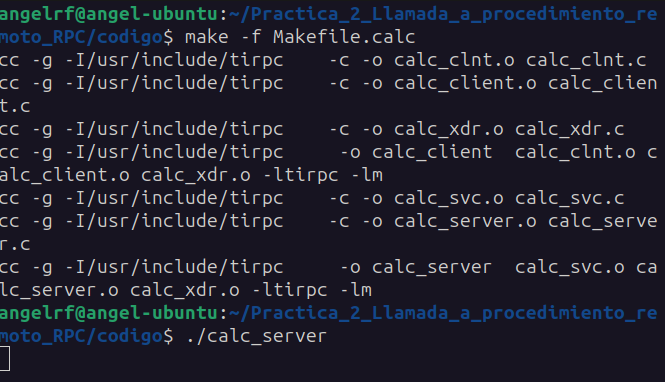
\includegraphics[width=\linewidth]{./imagenes_necesarias/lanzar_server.png}
			\end{minipage}
			
			\subsubsection{Ejecución del Cliente.}
				Con el servidor a la escucha, abrimos una segunda terminal para actuar como cliente. Recordamos que teníamos dos modos de funcionamiento, veamoslos por separado: 
				
				\begin{itemize}
					\item \textbf{Modo Terminal.} El primer modo de funcionamiento permite realizar cálculos rápidos pasando los parámetros directamente en la llamada al programa. la forma de llamarlo es:
						\begin{center}
							\fbox{\texttt{./calc\_client maquina numero operador numero}}
						\end{center}
					
					\textbf{Los operadores pueden ser: \texttt{$+$ $-$ $x$ $/$ $L$ $l$ $s$ $c$ $t$}}
			
					En la siguiente imagen se muestra un ejemplo donde se calcula la potencia ($2^8$):
					
					\begin{minipage}[c]{0.9 \textwidth}
						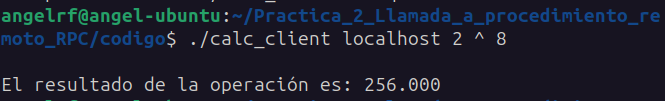
\includegraphics[width=\linewidth]{./imagenes_necesarias/ejemplo_2_elevado_8.png}
					\end{minipage}

					\item \textbf{Menú interactivo y Lotes.} Si el usuario desea una experiencia más guiada o necesita realizar múltiples cálculos a la vez de forma eficiente, invocará al cliente indicando únicamente la máquina servidor:
					
					\begin{center}
						\fbox{\texttt{./calc\_client localhost}}
					\end{center}
					
					Al hacerlo, el programa desplegará el menú interactivo. Si el usuario selecciona la opción correspondiente a las operaciones por lote, se activará la función \texttt{leer\_lote}, solicitando los datos de forma secuencial. Una vez recopilados, viajarán por la red en una única transacción y el cliente mostrará los resultados formateados.
					
					En la siguiente imagen se muestra un ejemplo del menú interactivo, junto a una petición de realizar una división (66 / 8):
					
					\begin{minipage}[c]{0.9 \textwidth}
						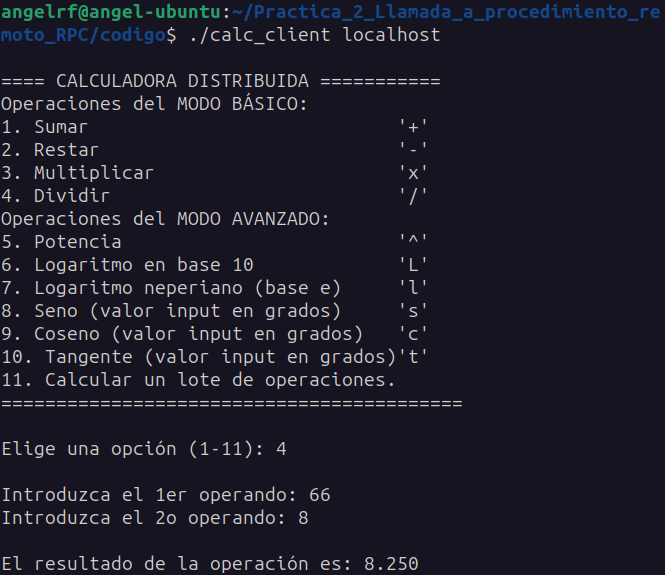
\includegraphics[width=\linewidth]{./imagenes_necesarias/ejemplo_menu_y_division.png}
					\end{minipage}
					
					\newpage
					
					Para finalizar, se muestra un ejemplo del calculo de un lote compuesto por 3 operaciones:
					
					\begin{minipage}[c]{1 \textwidth}
						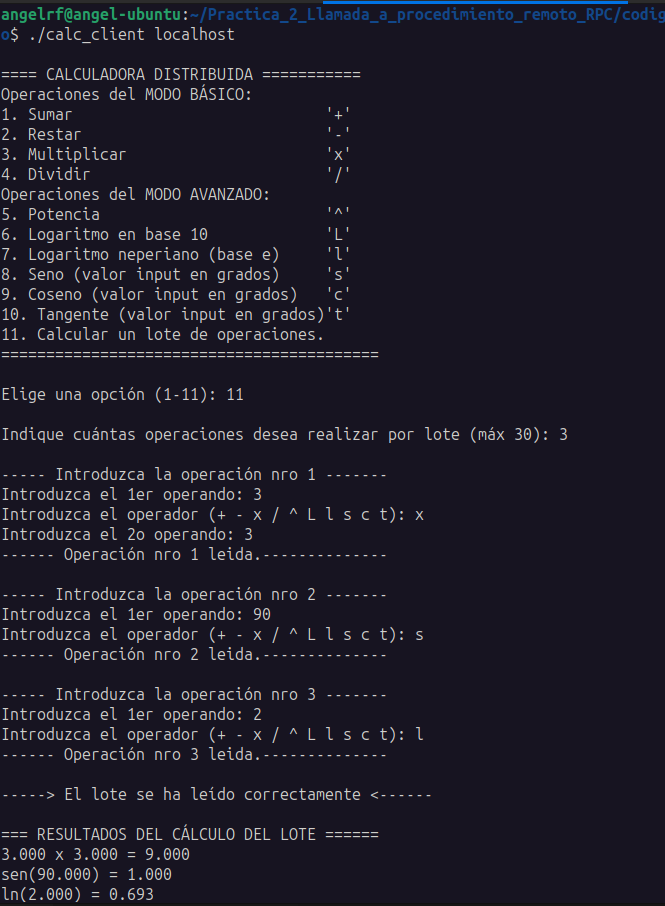
\includegraphics[width=\linewidth]{./imagenes_necesarias/ejemplo_calculo_por_lote.png}
					\end{minipage}
					
				\end{itemize}

\end{document}